\documentclass[a4paper]{article}
\usepackage{float}
\usepackage{geometry}
\usepackage{listings}
\usepackage{hyperref}
\usepackage{plantuml}
\usepackage{graphicx}
\usepackage{ragged2e}
\usepackage{color}
\usepackage{xepersian}
\usepackage{subfiles}
\newgeometry{left=1.4cm, right=1.4cm, bottom=2.0cm, top=2.0cm}
\settextfont[Scale=1]{XB Roya}

\title{نظریه پیچیدگی \footnote{\lr{Computational complexity theory}}}
\author{علیرضا سلطانی نشان}

\begin{document}
\maketitle
\tableofcontents

\section{مجوز}

به فایل license همراه این برگه توجه کنید. این برگه تحت مجوز GPLv3 منتشر شده است
که اجازه نشر و استفاده (کد و خروجی/pdf) را رایگان می‌دهد.

\section{پیش گفتار}

در حال خواندن مقاله‌ای در مورد طراحی دارو‌ها به وسیله ترکیب و اتصال پروتئین‌ها
بودم که متوجه شدم الگوریتم‌ها و قضیه‌هایی که در آن مطرح شده را نمی‌توانم متوجه
شوم، تصمیم بر آن گرفتم که یک جزوه ساده در مورد آن‌ها بنویسم. منابع مطالبی که
اینجا نگاشته شده است را در بخش مراجع می‌توانید مشاهده کنید. در صورت مغایرت با
مطالب درست می‌توانید آن را تصحیح نمایید.

\section{کلاس‌های پیچیدگی}

سطح دشواری یک مسئله را مشخص می‌کند. برای رسیدن به پاسخ یک مسئله چه دشواری‌هایی
را خواهیم داشت. برای حل هر مسئله به تعداد پیش‌نیاز‌ها احتیاج داریم:

منابع اصلی برای حل مسئله:

\begin{enumerate}
    \item زمان: مدت زمانی که می‌توانیم یک مسئله را دریافت کنیم و به پاسخ آن
    برسیم.
    \item فضا: برای حل مسئله چه پارامتر‌هایی بیان شده است؟ چه میزان حافظه برای
    رسیدن به پاسخ نیاز داریم؟
\end{enumerate}

پیچیدگی زمانی یا همان مرتبه اجرایی الگوریتم به منظور تعیین تعداد مراحل مورد نیاز
برای حل مسئله می‌باشد. علاوه‌بر این، مرتبه اجرایی به منظور تعیین مدت زمان مورد
نیاز برای تایید جواب استفاده می‌شود.

درجه سختی سوال در نظریه پیچیدگی مطرح می‌شود، اینکه چه مسئله‌ای قابل حل است و چه
مسئله‌ای را نمی‌توان حل کرد. معروف‌ترین کلاس‌های پیچیدگی \lr{P} و \lr{NP}
می‌باشد که مسئله را از نظر زمان مورد نیاز تقسیم می‌کنند.

\begin{figure}[H]
    \centering
    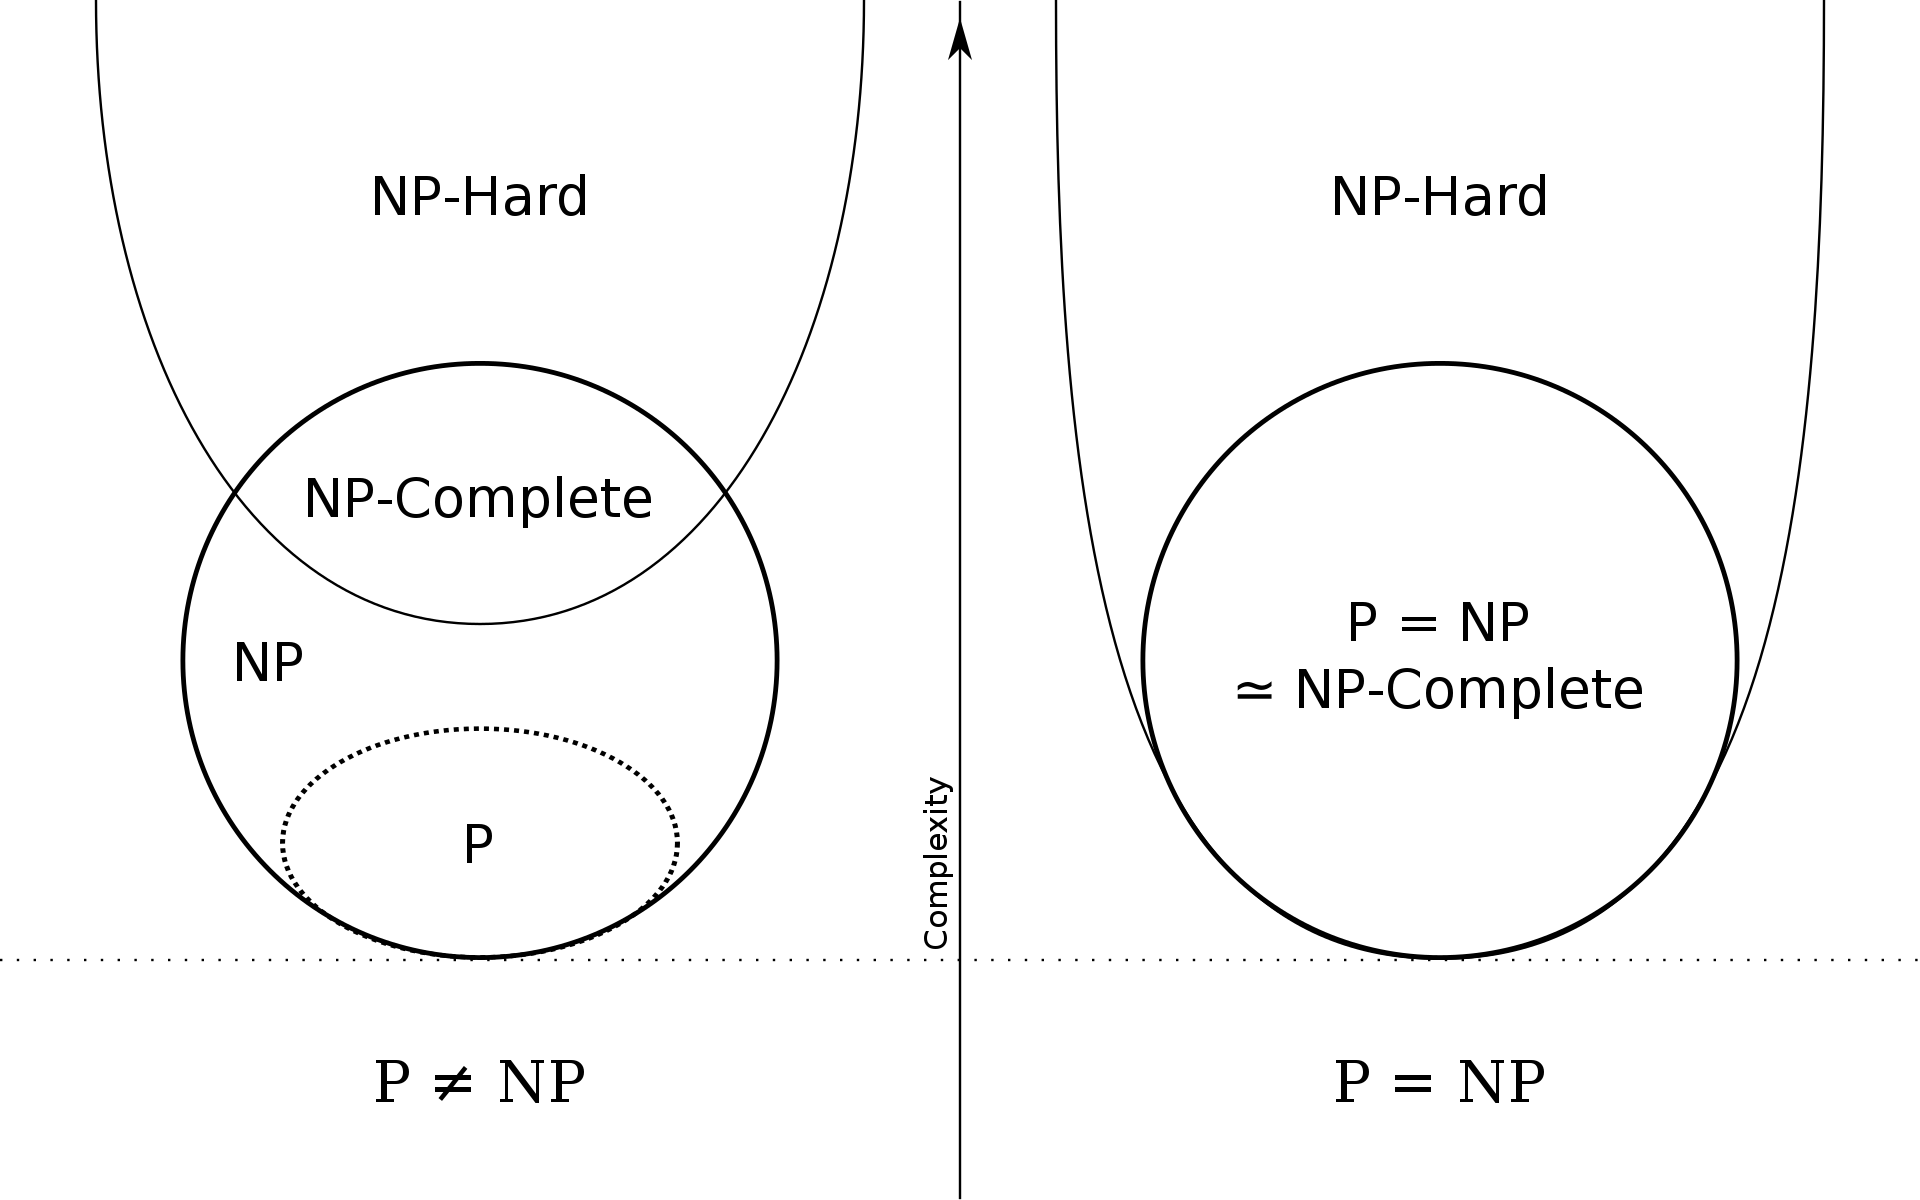
\includegraphics[width=0.6\textwidth]{images/euler_diagram.png}
        \caption{دیاگرام اویلر مسائل کلاس‌های پیچیدگی؛ از پایین به بالا ساده،
        متوسط، سخت، سخت‌ترین}
    \label{fig: uml}
\end{figure}

\subsection{کلاس \lr{P}}

\lr{P} یک کلاس پیچیدگی است که مجموعه‌ای از تصمیم‌گیری‌هایی که می‌توان در زمان حل
یک معادله چند جمله‌ای داشت را نشان می‌دهد. معمولاً پاسخ این مسائل به صورت بلی یا
خیر بیان می‌شود و توسط ماشین قطعی و در زمان چندجمله‌ای قابل حل است. برای مثال
مسئله زیر می‌تواند مطرح شود:

گراف \lr{G} را داریم، آیا می‌توان رئوس این گراف را به گونه‌ای رنگ آمیزی کرد که
هیچ لبه‌ای تک رنگ نباشد؟

الگوریتم آن در نظریه گراف: از یک راس دلخواه شروع می‌کنیم. آن را قرمز می‌کنیم و
تمام رئوس همسایه را آبی می‌کنیم و ادامه می‌دهیم. این عمل را تا جایی انجام
می‌دهیم که یال کشیده شده بین
رئوس جدید تک رنگ نباشد.

\subsubsection{ویژگی‌های کلاس \lr{P}}

\begin{enumerate}
    \item یافتن راه‌حل برای مسائل \lr{P} آسان است.
    \item مسائل \lr{P} اغلب قابل‌حل و رام‌پذیر (\lr{Tractable}) هستند. مسئله
    رام‌پذیر مسئله‌ای است که هم به صورت نظری هم به صورت عملی قابل حل می‌باشد.
    اما مسئله غیر رام‌پذیر دقیقا مسئله‌ای است که تنها در تئوری قابل حل و اثبات
    می‌باشد اما در عمل غیر قابل‌حل
\end{enumerate}

\subsubsection{کاربرد‌ها}

\begin{enumerate}
    \item محاسبه بزرگ‌ترین مقسوم علیه مشترک
    \item افتن حداکثر تطابق
    \item نسخه‌های تصمیم برنامه‌ریزی خطی
\end{enumerate}

\subsection{کلاس \lr{NP}}

\lr{NP} یک کلاس پیچیدگی است که مجموعه از پاسخ‌ها را به همراه مدارک و اثبات حل
مسئله را در صورتی که پاسخ مسئله بله باشد را ارائه می‌دهد. برای مثال مسئله زیر
می‌تواند مطرح شود:

فرض کنید که یک لعتنامه با تعداد کلمات محدود دارید. می‌خواهیم با استفاده از ترکیب
این لغات به یک کلمه ۱۰ حرفی مشخص برسیم. آیا این ترکیب امکان پذیر است؟ اگر راه‌حل
این مسئله مشخص است، آن را می‌نویسم، اما اگر مشخص نیست تماماً باید با مدارک و
شواهد ثابت گردد که این لغتنامه محدود مناسب ساخت این ترکیب نیست.

\subsection{کلاس \lr{NP-Complete}}

\subsection{کلاس \lr{NP-Hard}}

\subsection{قضیه $P = NP$}

\end{document}
